\title{Implementation of associative array in \CC{} using Trie data structure}
\author{
        %\large
        \textsc{MICHAL KARPINSKI}
        \mbox{}\\ %
        Institute of Computer Science\\
        University of Wroclaw\\
        \mbox{}\\ %
        \normalsize
            \texttt{karp0506@gmail.com}
}
\date{\today}
\documentclass[a4paper,12pt]{article}

\usepackage[dvips,top=2cm,left=2cm,right=2cm,
    foot=1cm,bottom=2cm]{geometry}


\usepackage[fleqn]{amsmath}
\usepackage{amsfonts}
\usepackage{amssymb}
\usepackage{amsthm}
%\usepackage{amsopn}
\usepackage{xspace}
\usepackage[utf8]{inputenc}
%\usepackage[OT4]{fontenc}
\usepackage{graphicx}
\usepackage{multirow}

\newcommand\CC{\Lang{\mbox{C++}}\xspace}
\newcommand\Lang[1]{\textsc{#1}}

%\usepackage{labels}

\setcounter{topnumber}{0}
\setcounter{bottomnumber}{0}
\setcounter{totalnumber}{20}
%\renewcommand{\textfraction}{0.01}

%\linespread{1.0}

\newtheorem{defi}{Definition}
\newtheorem{theo}[defi]{Theorem}
\newtheorem{lemma}[defi]{Lemma}
\newtheorem{obs}[defi]{Observation}

\begin{document}

\maketitle

\begin{abstract}
This paper introduces simple yet powerful data structure
    called trie tree and its use in building an \emph{associative array} - an
    abstract data type composed of a collection of unique keys and a
    collection of values, where each key is associated with one value.
Such data structure is often called \emph{dictionary} or \emph{finite map}.
\end{abstract}

\section{Introduction}
In standard library of \CC{} there already is a container that would work as a
    good associative array - it's called \emph{map} and it's an implementation 
    of balanced tree.
The question that first comes to mind is: "Why would we want
    to recreate something that already exists?".
While \emph{map} is indeed a wonderful container - good for general uses - it has one weakness
    which we are going to exploit in order to beat it with our implementation.
That weakness comes to play when we are using \emph{strings} as keys. 
In general we want to store words over some finite alphapet $\Sigma$.

In balanced tree we would store each word in one node. This will suffice when we assume that
the size of each word is bound by some constant. Then the time complexity of single query is
$O(\log n)$ (where $n$ is number of words). It is not so simple if we do not know the size of words beforehand
(which is usually the case). Time complexity for one query rises to $O(m\log n)$ (where $m$ is length of word).

This paper shows superiority of trie tree over \emph{map} when working with keys that are words. 
By using mathematical proofs and practical experiments we will see that our associative array 
beats the time complexity of the balanced tree.

\subsection{Contents}

The main body of this paper is divided as follows.

Chapter 2 covers theoretical knowledge about tire. This is where the trie structure is explained.
In this chapter we will also learn how the basic dictionary operations work.
As an nessesery addition every aspect of the structrue has approperiate corretness and complexity proof.

In Chapter 3 we enter the world of \CC{} and see how to easily implement trie tree for our assosiative array.
This is where the parts of code is presented and explained simultaneously.

The results of experiments using the program included with this paper are presented in next Chapter 4.
Here we compare our implementation of associative array with the \emph{std::map} container in practical use. 

The last chapter summarizes entire study.
\section{Trie}

Let's begin with a general definition of trie:

\begin{defi}
Given alphabet $\Sigma$ and a collection of words $W$ over that alphabet, $T(W)$ is the trie of words $W$.
Trie is a rooted tree in which each node stores one letter that occurs in one (or more) words from $W$. We say that node $v$ is assosiated with word $w$ when word read after going down a path from the root to the node $v$ is $w$. All the descendants of a node have a common prefix of the word associated with that node, and the root is associated with the empty string. 
\end{defi}

\begin{figure}[ht]
\begin{center}
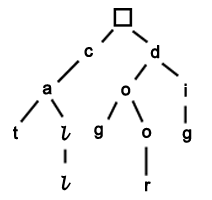
\includegraphics[scale=0.60,angle=0]{trie1.png}
\caption{Example of trie}
\end{center}
\end{figure}

Definition of trie may seem a little bit complicated so let's look at the simple example in figure 2.1. It presents the trie bulit from words: \emph{\{cat, call, dog, door, dig\}}. We can see that retrieving every word from that structure is rather easy: we just have to go down the path - starting from root (represented by top square) - collecting letters that will form our words when we reach every leaf. We will be using that example through the rest of this paper.

We can already get some useful information from our definition:

\begin{obs}
Maximum number of childeren of a single node is $|\Sigma|$ 
\end{obs}

\noindent Which leads us to an obvious conclusion that:

\begin{obs}
Assuming fixed size of alphabet $\Sigma$, time to look through all children of a given node is $O(1)$.
\end{obs}

\noindent Now let's see how basic dictionary operations are performed on trie.

\subsection{Lookup}

To check if trie $T$ contains word $w$ we use operation $LookUp(w,root(T))$. (Note that $root(T)$ is a pointer to the root of trie $T$, $char(v)$ is letter stored in node $v$). $LookUp$ can be writen as a recursive function:


\begin{itemize}
\item {\em LookUp(w,v):}
	\begin{enumerate}
	\item {\bf if} $w$ is empty {\bf then} {\bf return} {\bf v} 
	\item $c  \gets w[1]$
	\item $w' \gets w[2..length(w)]$
	\item $u  \gets$ child of $v$ such that $char(v)=c$
	\item {\bf if} $u$ exists {\bf then} {\bf return} {\em LookUp(w',u):}
	\item {\bf else} {\bf return} {\bf NULL}
	\end{enumerate}
\end{itemize}

The pseudo-code above is self-explanatory. 

\subsection{Insertion}

Insertion is also presented by a recursive function: 

\begin{itemize}
\item {\em Insert(w,v):}
	\begin{enumerate}
	\item {\bf if} $w$ is empty {\bf then} {\bf exit} 
	\item $c  \gets w[1]$
	\item $w' \gets w[2..length(w)]$
	\item $u  \gets$ child of $v$ such that $char(v)=c$
	\item {\bf if} $u$ exists {\bf then} {\bf return} {\em Insert(w',u)}
	\item {\bf else}
	\item . . Create new node $u$ with $char(u)=c$
	\item . . Add $u$ as a new child of $v$ 
	\item . . {\bf return} {\em Insert(w',u)}
	\end{enumerate}
\end{itemize}

This procedure is very similar to the {\em LookUp}. Extending our dictionary by another word $w$ begins at the root of trie. New word may contain a preffix of some words that are already stored in our tree. We go down the trie discarding front letters of $w$ until we find a node where that preffix ends. From this node we will create new nodes for the rest of word $w$ by tying them up with parent-child relationship.

\subsection{Deletion}

Here is a pseudo-code for removing a word from a tire. Note that this procedure is not recursive.

\begin{itemize}
\item {\em Remove(w,T):}
	\begin{enumerate}
	\item $node \gets$ {\em LookUp(w,root(T))}
	\item {\bf if} $node$ is {\bf NULL} {\bf then} {\bf exit}  
	\item {\bf while} $node$ doesn't have children {\bf AND} $node != root(T)$ {\bf do}
	\item . . $x \gets$ parent of $node$
	\item . . Delete $node$
	\item . . $node \gets x$ 
	\end{enumerate}
\end{itemize}

Deleting word $w$ consists of two steps. Step 1: find the node $v$ that represents word $w$. If such node does not exist, then we have nothing to remove. Step 2: delete all nodes from bottom to top: staring at node $v$, going up through parent-child relationship, ending at the first node that have at least one child (or at root).

\subsection{Correctness proof}

Corretness proof for all the procedures that were given above is solved by simple induction which I will leave for the reader.

\subsection{Time complexity}

\begin{theo}
Given word of length $m$ over fixed sized alphabet $\Sigma$, every basic dictionary operation on trie can be done in $O(m)$ time.
\end{theo}

\begin{proof}
Number of operations that are performed during one recursive call in $Insert$ and $LookUp$ is constant. Number of recursive calls is at most $m$ which ends the proof. As for $Delete$ procedure: first step takes $O(m)$ time. For the second step: the $while$ loop iterates at most $m$ times. \qedhere
\end{proof}


\section{Implementation in C++}

Finally we got to the core of this paper. Here the implementation details will be presented. The trie can be constructed by connecting nodes using pointers to another nodes. Let's define what a single node contains:

\begin{figure}[!htb]
\begin{tabbing}
stru\=ct trie\_node \{ \\
\>    trie\_node * next; \\
\>    trie\_node * left; \\
\>    trie\_node * right; \\
\>    trie\_node * parent; \\
\>		char c;	\\ 
\>		T * value; \\
\};
\end{tabbing}
\end{figure}

\begin{figure}[ht]
\begin{center}
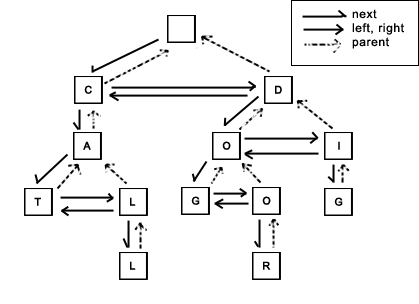
\includegraphics[scale=0.65,angle=0]{trie2.png}
\caption{Node links}
\end{center}
\end{figure}

Consider we have constructed node $v$. From top to bottom: \emph{v$->$next} points at a left-most child of node $v$; \emph{v$->$left} and \emph{v$->$right} pointers form a part of doubly-linked list of brothers of node $v$. Meaning of the last pointer \emph{v$->$parent} is obvious. We also have letter $c$ and a pointer to $value$ of type $T$. This type can be anything. We can even make template out of this structure (which is recommended) but to keep things simple we will omit unnecessary decalarations. Figure 2 presents nodes with pointers in our example ($NULL$ pointers were omitted).

The value pointer (if it's not $NULL$) also indicates that the word associated with node $v$ belongs to the trie. This is useful because some words in the trie can end at internal node, not always at leaf. Such situation happens when a certian word is a preffix of some other word that belongs to the same trie (Ex.: \emph{do},\emph{door}).

The most importnant thing about the \emph{v$->$value} is that it's the only addition we need to the trie structure that will be needed to form an associative array.

Let's define the trie structure. Definition of constructors and destructor is left for the reader to write. We just have to remember make the $root$ pointers $NULL$ at the beginning and write approperiate recursive procedure for freeing allocated memory. The structure looks like this:

\begin{figure}[!h]
\begin{tabbing}
stru\=ct trie \{ \\
\>    trie * root; \\
\>	\\
\>		/* basic procedures */ \\
\>		trie\_node * lookup(const char word []); \\
\>		bool insert(const char word [], T\& v); \\
\>		bool remove(const char word []); \\
\>	\\	
\>		T\& g\=et(const char word []) \{ \\
\> \>				trie\_node node = lookup(word); \\
\> \>				return ( node ? node$->$v : 0 ); \\
\>		\} \\
\};
\end{tabbing}
\end{figure}

Again, starting from the top: the trie has its $root$. Next we see declarations of three basic dictionary operations: $lookup$, $insert$ and $remove$. In the bottom we see definiotion of method \emph{get(const char word [])} which returns value assosiated with the $word$ (if it has one).

There is nothing unusual about the structure so let's get straight to the implementation of our first known method: $lookup$. For starters:

\begin{figure}[!h]
\begin{tabbing}
trie\=\_node * trie::lookup( const char word [] ) \{ \\
\>  trie\_node * act = root; \\
\>  int word\_len = \emph{strlen(word)}; \\
\>  int i = 0; \\
\end{tabbing}
\end{figure}

\noindent This is the beginning of $lookup$s body. Here we define some auxiliary variables: $act$ (as in $active$) is a pointer to the node we are currently in. We begin from the $root$. Next we have two variables of type $int$: $word\_len$ which is length of $word$ and $i$ - for iterating through $word$. Let's begin the iteration: 

\newpage

\begin{figure}[!h]
\begin{tabbing}
\quad \quad \= \\
\> whil\=e( act$->$next ) \{ \\
\> \>    act = act$->$next; \\
\end{tabbing}
\end{figure}

\noindent If \emph{act$->$next} is not $NULL$ then $act$ has at least one child. We jump to the left-most child of $act$.

\begin{figure}[!h]
\begin{tabbing}
\quad \quad \quad \quad \= \\
\>    whil\=e ( act$->$c != word[i] \&\& act$->$right != 0) \{ \\
\> \>     act = act$->$right; \\
\>    \} \\
\end{tabbing}
\end{figure}

\noindent This loop iterates through brothers of $act$ (from left to right) and stops until we find node with letter equal to $word[i]$ (or at the end of brothers list).

\begin{figure}[!h]
\begin{tabbing}
\quad \quad \quad \quad \= \\
\>    if (\= act$->$c != word[i] ) \{ \\
\> \>      return 0; \\
\>    \} \\
\end{tabbing}
\end{figure}

\noindent If above condition is true then we looked through all brothers and did not find the needed node. It means the $word$ is not in the trie. We return a $NULL$ pointer.

\begin{figure}[!h]
\begin{tabbing}
\quad \quad \quad \quad \= \\
\>   i++; \\
\end{tabbing}
\end{figure}

\noindent Now we can increment $i$ thus consider the next letter of $word$. But we have to make one final check:

\begin{figure}[!h]
\begin{tabbing}
\quad \quad \= \quad \quad \= \\
\>\>    if (\= i == word\_len ) \{ \\
\>\>\>      if (\= act$->$value ) \\
\>\>\>\>        return act; \\
\>\>\>      else \\
\>\>\>\>        return 0; \\
\>\>    \} \\
\>  \} // end of while loop \\
\end{tabbing}
\end{figure}

\newpage

\noindent If we are done reading the word, then either there is some value assosiated with the current node or not. In the first case we return pointer to this node. In the second case we return $NULL$.

\begin{figure}[!h]
\begin{tabbing}
\quad \quad \= \\
\>  return 0; \\
\} \\
\end{tabbing}
\end{figure}

\noindent If we finished the main loop, that means we are in some leaf that does not represent the $word$, so we return $NULL$.

That is all for the lookup. Now we will define insertion which is very similar to lookup, but with minor changes. 

\begin{figure}[!h]
\begin{tabbing}
bool\= \quad trie::insert ( const char word [], T\& v ) \{ \\
\>  trie\_node * act = root; \\
\>  int word\_len = \emph{strlen(word)}; \\
\>  int i = 0; \\
\> \\
\>  whil\=e ( act$->$next ) \{ \\
\>\>    act = act$->$next; \\
\>\> \\
\>\>   whil\=e ( act$->$c != word[i] \&\& act$->$right != 0) \{ \\
\>\>\>    act = act$->$right; \\
\>\>    \} \\
\end{tabbing}
\end{figure}

\noindent As we can see - beginning does not change.

\begin{figure}[!h]
\begin{tabbing}
\quad \quad \quad \quad \= \\
\>    if (\= act$->$c != word[i] ) \{ \\
\>\>      trie\_node * node = new trie\_node ( word[i] ); \\
\>\>      act$->$right = node; \\
\>\>      node$->$left = act; \\
\>\>      node$->$parent = act$->$parent; \\
\>\>      act = act$->$right; \\
\>    \} \\
\end{tabbing}
\end{figure}

\noindent Here we can see the first difference. If we can't find letter $word[i]$ in brothers list, we have to create new node with that letter.

\newpage

\begin{figure}[!h]
\begin{tabbing}
\quad \quad \= \quad \quad \= \\
\>\>   i++; \\
\>\>	\\
\>\>   if (\= i == word\_len ) \{ \\
\>\>\>      if (\= act$->$value ) \\
\>\>\>\>        return false; \\
\>\>\>      else \{ \\
\>\>\>\>     	act$->$value = v; \\
\>\>\>\>     	return true; \\
\>\>\>     \} \\
\>\>    \} \\
\>  \} // end of while loop \\
\end{tabbing}
\end{figure}

\noindent Again we see similarity to the lookup method. The diffrence is when a node that represents $word$ already has a value assosiated with it, then we do nothing and return $FALSE$, otherwise we assign $v$ with to \emph{act$->$value} and return $TRUE$.

\begin{figure}[!h]
\begin{tabbing}
\quad \quad \= \\
\> whil\=e ( i $<$ word\_len ) \{ \\
\>\>    trie\_node * node = new trie\_node ( word[i] ); \\
\>\>    act$->$next = node; \\
\>\>    node$->$parent = act; \\
\>\>    act = act$->$next; \\
\>\>    i++; \\
\>  \}
\> \\
\>  act$->$value = new T(value); \\
\> \\
\>  return true; \\
\} \\
\end{tabbing}
\end{figure}


\noindent After leaving the loop we are in leaf that represents the prefix of word = word[1..i] which is already inside the tire. We need to create more nodes and complete insertion.

The only thing that is left for us to define is remove method. Let's begin:

\begin{figure}[!h]
\begin{tabbing}
bool\= \quad trie::remove( const char word [] ) \{ \\
\>  trie\_node * del = \emph{lookup ( word )}; \\
\>  trie\_node * tmp; \\
\>  if ( ! del ) return false; \\
\end{tabbing}
\end{figure}

\noindent Variable $del$ points to the node that represents the $word$. If such node doesn't exist, then we have nothing to delete, so we finish the procedure.

\newpage

\begin{figure}[!h]
\begin{tabbing}
\quad \quad \= \\
\>  whil\=e( del$->$parent \&\& !(del$->$right $||$ del$->$left) ) \{ \\
\>\>    tmp = del$->$parent; \\
\>\>    delete del; \\
\>\>    del = tmp; \\
\>  \} \\
\end{tabbing}
\end{figure}

\noindent In this loop we are removing nodes from trie bottom-up until we encounter the node with at lest one child.

\begin{figure}[!h]
\begin{tabbing}
\quad \quad \= \\
\>  if (\=del == root) \{ \\
\>\>    root$->$next = 0; \\
\>\>    return true; \\
\>  \} \\
\end{tabbing}
\end{figure}

\noindent Of course while removing the elements in previous loop we can even go up to the root. In this case the trie will be empty after deletion. There is nothing left to do so we finish the procedure.

\begin{figure}[!h]
\begin{tabbing}
\quad \quad \= \\
\>  if (\= del$->$left ) \{ \\
\>\>    tmp = del$->$left; \\
\>\>    tmp$->$right = del$->$right; \\
\>  \} else \{ \\
\>\>    tmp = del$->$parent; \\
\>\>    tmp$->$next = del$->$right; \\
\>\>    tmp$->$next$->$left = 0; \\
\>  \} \\
\end{tabbing}
\end{figure}


\noindent In this (and next) conditional statement we are fixing the pointers to the left and right brother of last node that we are going to delete.

\begin{figure}[!h]
\begin{tabbing}
\quad \quad \= \\
\>  if(\= del$->$right ) \{ \\
\>\>    tmp = del$->$right; \\
\>\>    tmp$->$left = del$->$left; \\
\>  \} \\
\end{tabbing}
\end{figure}

\noindent After this fix there is only one thing to do:

\newpage

\begin{figure}[!h]
\begin{tabbing}
\quad \quad \= \\
\>  delete del; \\
\>  return true; \\
\} \\
\end{tabbing}
\end{figure}

\noindent Lets continue to the practical part of this paper.

\section{Experiments}

The experiment will be simple. We will compare two data structures: $RedBlackTree$ and $Trie$. The results will be presented in table below. The input data is a set of randomly generated words of random length (from $20$ to $40$ characters each). In each step of the experiments the set will grow larger up to some reasonable size. First we will see how fast each data structure is able to construct a dictionary from given set. Then we will delete every element of this dictionary and see which is going to be emptied faster.

\begin{center}
\begin{tabular}{|l|l|l|l|l|} \hline
\multirow{2}{*}{Size} & \multicolumn{2}{|c|}{Insert} & \multicolumn{2}{|c|}{Delete} \\ \cline{2-5}
& Trie & RBTree & Trie & RBTree \\ \hline
$10^3$ 				& $0.008$  & $0.006$  & $0.005$ & $0.003$ \\ \hline
$10^4$ 				& $0.076$  & $0.079$  & $0.011$ & $0.005$ \\ \hline
$10^5$ 				& $0.880$  & $0.750$  & $0.277$ & $0.052$ \\ \hline
$10^6$ 				& $8.345$  & $9.593$  & $1.030$ & $0.540$ \\ \hline
$2\cdot 10^6$ & $17.744$ & $20.555$ & $3.354$ & $1.342$ \\ \hline
\end{tabular}
\end{center}

All the values in the table are given in seconds. This mesures the time needed to complete each task for given set size. The experiment was performed multiple times and every result presented in the table above is the avarage of all the experiments.

The results are satisfactory. As we can see, for small sets, both data structures are performing equally good. But as the set grow larger the insertions in $Trie$ are being caried out faster. As for the clean-up: $RBTree$ wins here, but this is not odd behavior since keys in $RBTree$ are stored in memory as continuous blocks of data and it is easy to delete them. In the $Trie$ keys are dismantled so removing each value is obviously slower.

\section{Summary}

From what was presented in this paper we can conclude, that trie is perfect for storing static dictionaries (such as telephone book) where only importnant operations are insertions and lookups. Our implementation was constructed as a dynamic data structure that also can perform deletion, but simple modifications would give more saved memory.

For general uses I still recommend STLs $map$, but one might consider using more specialized data structure (like Trie) for given problems.

\end{document}